\documentclass[10pt,twocolumn]{article}
\usepackage[margin=0.72in]{geometry}
\usepackage{graphicx,booktabs,microtype,natbib,url,xcolor}
\usepackage[T1]{fontenc}
\usepackage{lmodern}
\setlength{\columnsep}{0.22in}
\newcommand{\system}[1]{\texttt{#1}}
\newcommand{\PlainAcc}{54.2}
\newcommand{\PlainLo}{39.6\%}
\newcommand{\PlainHi}{68.8\%}
\newcommand{\PlainP}{0.665}
\newcommand{\OutlineAcc}{50.0}
\newcommand{\OutlineLo}{39.6\%}
\newcommand{\OutlineHi}{60.4\%}
\newcommand{\OutlineBinomP}{1.000}
\newcommand{\DistractorAcc}{41.7}
\newcommand{\DistractorLo}{29.2\%}
\newcommand{\DistractorHi}{54.2\%}
\newcommand{\DistractorP}{0.312}
\newcommand{\DecoyAcc}{39.6}
\newcommand{\DecoyLo}{27.1\%}
\newcommand{\DecoyHi}{52.1\%}
\newcommand{\DecoyP}{0.193}
\newcommand{\OutlineDiff}{--4.2}
\newcommand{\OutlineDiffLo}{--22.9}
\newcommand{\OutlineDiffHi}{14.6}
\newcommand{\OutlineP}{0.836}
\newcommand{\DistractorDiff}{--12.5}
\newcommand{\DecoyDiff}{--14.6}
\newcommand{\MainFindingSentence}{the plain positive anchor itself is statistically indistinguishable from chance, so the data do not identify an outline-specific reduction}
\newcommand{\BehaviorResultParagraph}{The plain condition is only 54.2\%, and its interval includes chance. Outline accuracy is exactly 50.0\%; distractor and decoy point estimates are below chance, but neither differs significantly from chance. Thus the planned positive anchor failed in this constrained-premise protocol}
\newcommand{\ConfoundConclusion}{neither a planning benefit nor a dilution account is identified: the assay is at a behavioral floor before either explanation can be separated}
\newcommand{\LiteralCompliance}{100.0}
\newcommand{\LiteralCount}{zero}
\newcommand{\MinWords}{265.3}
\newcommand{\MaxWords}{285.7}
\newcommand{\QualityGap}{0.17}
\newcommand{\ProbeAcc}{20.8}
\newcommand{\ProbeLayer}{48}
\newcommand{\ProbeQuartile}{2}
\newcommand{\ProbeFinalAcc}{9.7}
\newcommand{\ProbeRho}{0.059}
\newcommand{\ProbeP}{0.623}
\newcommand{\ProbeAboveChanceDescription}{no depth--quartile cell robustly above chance after accounting for the 28 inspected cells}
\newcommand{\ProbeInterpretation}{The isolated maximum has an uncorrected binomial $p=0.047$, but it does not survive even a simple multiplicity correction, final-quartile performance is at chance, and behavioral correlation is absent}
\newcommand{\AblationAcc}{6.3}
\newcommand{\AblationLo}{0.0\%}
\newcommand{\AblationHi}{12.5\%}
\newcommand{\RandomAcc}{56.3}
\newcommand{\RandomLo}{43.8\%}
\newcommand{\RandomHi}{68.8\%}
\newcommand{\AblationDiff}{--50.0}
\newcommand{\AblationP}{<0.001}
\newcommand{\AblationQuality}{1.23}
\newcommand{\RandomQuality}{4.02}
\newcommand{\AblationConclusion}{Projection of the prompt contrast catastrophically damages generation (98 versus 273 mean words, with many malformed or multilingual token sequences). Its below-chance detection is therefore a distributional collapse, not evidence of selective secret removal}
\newcommand{\DiscussionParagraph}{The central result is an informative failure of identification. Although earlier work found strong leakage from Gemma~3 12B when the model freely chose a story, our plain condition fixes a premise and produces only 54.2\% detection. The most plausible design-level difference is that even a short premise already constrains content selection, leaving little measurable leakage for a fuller outline to remove. The data therefore do not support the headline causal hypothesis, but neither do they show that plans are ineffective when leakage is present}
\newcommand{\ConclusionParagraph}{Under fixed premises, Gemma~3 12B did not provide the required above-chance leakage anchor. Outlines, irrelevant context, and decoys all yielded estimates compatible with chance, and secret identity was not robustly decoded from story-period residual states. The correct conclusion is not that outlines solve leakage, but that premise-constrained generation can create a floor that makes the comparison uninformative}

\title{Can a Plan Keep a Secret?\\Explicit Outlines and Involuntary Leakage in Language-Model Fiction}
\author{Anonymous}
\date{}
\begin{document}
\maketitle

\begin{abstract}
Language models instructed not to reveal a secret can nevertheless let it influence their writing. We test a proposed explanation: prose leaks because content planning and realization are entangled, so supplying a plan should reduce leakage. Gemma~3 12B writes 192 stories in 96 matched secret/no-secret pairs spanning eight secret words, three premises, and four conditions: plain, a secret-independent outline, length-matched irrelevant context, and a decoy concept. A position-balanced GPT-4.1-mini judge identifies the secret-conditioned story with \PlainAcc\% accuracy in the plain condition. An explicit outline yields \OutlineAcc\% (difference \OutlineDiff\ percentage points, paired randomization $p=\OutlineP$), while irrelevant context yields \DistractorAcc\% and a decoy yields \DecoyAcc\%. Thus, in this sample, \MainFindingSentence. Cross-premise linear probes do not robustly decode which of eight secrets was present from story-period residual states: the best of 28 inspected depth--time cells reaches \ProbeAcc\% (chance 12.5\%) but does not survive multiplicity correction. Probe confidence and behavioral leakage correlate at only $\rho=\ProbeRho$ ($p=\ProbeP$). Projecting out a prompt-derived direction at layer 24 drives detection to \AblationAcc\%, but also collapses quality from \RandomQuality\ to \AblationQuality\ out of five relative to random-direction removal, making the causal result uninterpretable. The outcome is a useful null: a fixed premise can remove the positive anchor needed to identify whether a fuller plan helps.
\end{abstract}

\section{Introduction}
A model may obey the literal instruction ``do not say the secret'' while its choices of setting, imagery, and topic reveal what it knows. \citet{holtzman2026secret} recently quantified this phenomenon: another model could discriminate secret-conditioned fiction at rates far above chance even when the word itself never appeared. Their results establish a behavioral effect but leave a natural mechanistic question. Is leakage partly a consequence of asking one autoregressive process to decide what happens and realize those decisions as prose while keeping a forbidden concept active?

We test the concrete prediction that an external, secret-independent outline reduces leakage. This intervention has a serious confound: any additional text may merely dilute the secret in a longer prompt. We therefore compare the outline against length-matched editorial instructions that constrain form but not story content. We also include a plain positive anchor and a decoy concept, a mitigation shown to redirect leakage \citep{holtzman2026secret}. Every secret story is paired with a separately sampled story from an otherwise identical prompt with no secret; this controls for what a premise makes guessable on its own.

Our second question is whether secret identity is recoverable from the writer's residual stream during the story. We extract states at seven depths and four temporal bins, training eight-way probes with entire premises held out. Finally, we perform an explicitly exploratory causal test: at layer 24, we project away the contrast between the final prompt state with and without a secret, with a norm-matched random direction as control.

The experiment gives three contributions. First, it is a controlled test of outlines rather than a replication alone. Second, it separates content fixation from prompt length. Third, it connects matched behavioral trials to internal measurements in an open-weight model. Our evidence is intentionally scoped to one writer and one automated reader; it supports claims about this evaluation, not universal model psychology.

\section{Related Work}
\paragraph{Semantic and privacy leakage.}
Semantic leakage is the intrusion of task-irrelevant prompt associations into generation \citep{gonen2025semantic}. Contextual-integrity evaluations instead ask whether models explicitly disclose private information in context \citep{mireshghallah2024secret}. Our setting concerns involuntary thematic evidence despite literal nondisclosure. \citet{holtzman2026secret} introduced the closest writer--guesser protocol, finding strong leakage in several frontier models, a size threshold within Gemma and Llama families, below-chance ``active hiding,'' and redirection by decoys. Ironic-negation work similarly finds rebound after ``do not think of'' instructions \citep{mann2025bear}, while \citet{baldelli2026hangman} formalize limits of secrecy without private working memory.

\paragraph{Planning and internal knowledge.}
Hidden states can encode global attributes of future responses \citep{dong2025planning}; other evidence distinguishes genuine pre-caching from representations useful both now and later \citep{wu2024future}. Explicit iterative plans improve suspenseful story generation \citep{xie2024suspense}, but leakage was not measured. Taboo model organisms show that logit lenses and sparse autoencoders can recover a fine-tuned hidden word \citep{cywinski2025latent}; our secret is supplied at inference time and the writer is asked to produce unrelated prose. Linear decodability is not itself proof of use \citep{hewitt2019probes}, motivating our separate, limited intervention.

\section{Method}
\subsection{Matched writer--guesser design}
The writer is the instruction-tuned, open-weight Gemma~3 12B model \citep{gemma2025report}, loaded in NF4 4-bit quantization. We use eight words from the original benchmark: \emph{umbrella, lighthouse, violin, cactus, telescope, nostalgia, copper, invoice}. They span concrete, abstract, and relatively neutral concepts. Each word is crossed with three fixed premises and four conditions, giving 96 secret/no-secret pairs (192 stories). Sampling uses temperature 0.8, top-$p$ 0.95, and fixed recorded seeds. Stories are requested at 260--320 words.

The secret prompt says that the model is privately holding word $w$ and must neither mention nor hint at it. The matched control replaces that sentence with a no-secret instruction. The conditions are:
\begin{description}
\item[Plain:] no added material.
\item[Outline:] a premise-specific, secret-independent four-beat content outline fixing opening, middle, turn, and ending.
\item[Distractor:] editorial directions matched approximately to outline length but not fixing content.
\item[Decoy:] a fixed unrelated concept on which imagery and incidental details should focus. The same decoy appears in the matched no-secret prompt.
\end{description}

GPT-4.1-mini \citep{openai2025gpt41}, accessed through OpenRouter, receives the secret and the two stories and chooses which writer knew it. Every pair is evaluated in both orders at temperature zero, yielding 48 judgments per condition. The judge also scores each story's quality from 1--5. Our estimand is pair-level accuracy averaged over the two orders. We report nonparametric 95\% bootstrap intervals over the 24 pairs. Condition contrasts are paired by secret and premise and use 200,000 sign-flip randomizations. Two-sided binomial tests over order-level decisions are descriptive because the two orders of a pair are dependent.

\subsection{Residual-stream probes}
For every secret-conditioned story, we teacher-force the stored prompt and generated text. We mean-pool residual states within each story quartile at the embedding output and after layers 8, 16, 24, 32, 40, and 48. We exclude the decoy condition because each secret has a deterministic decoy, which would make identity decoding tautological. At each layer/quartile, a standardized, 32-component PCA plus multinomial logistic regression predicts the eight-way secret identity; PCA is fit inside each fold. Three-fold cross-validation holds out one premise at a time, so a probe cannot solve the task by memorizing a secret's realization in the same premise. We use held-out true-class probability as a per-story representation-strength score and correlate it with behavioral accuracy. These states include the generated prefix, so decoding may reflect both latent memory and already-expressed textual associations.

\subsection{Exploratory directional ablation}
For each of the 24 plain secret--premise combinations, we take the difference between the final-prompt residual state with and without the secret after layer 24. During a fresh secret-conditioned generation, a forward hook removes the projection onto this unit direction from every layer-24 residual vector. A Gaussian direction orthogonalized against the secret direction serves as a random control. Both interventions use the same per-item sampling seed. Each output is compared with the original matched no-secret story in both presentation orders. This intervention targets a prompt contrast, not a uniquely identified semantic feature; we treat it as exploratory.

\section{Results}
\subsection{Behavioral leakage}
\begin{table}[t]
\centering
\caption{Position-balanced leakage detection. Accuracy averages the two orders for each matched pair; intervals bootstrap pairs.}
\label{tab:main}
\begin{tabular}{lccc}
\toprule
Condition & Pairs & Accuracy (95\% CI) & Binomial $p$\\
\midrule
Plain & 24 & \PlainAcc\% [\PlainLo, \PlainHi] & \PlainP\\
Outline & 24 & \OutlineAcc\% [\OutlineLo, \OutlineHi] & \OutlineBinomP\\
Distractor & 24 & \DistractorAcc\% [\DistractorLo, \DistractorHi] & \DistractorP\\
Decoy & 24 & \DecoyAcc\% [\DecoyLo, \DecoyHi] & \DecoyP\\
\bottomrule
\end{tabular}
\end{table}

Figure~\ref{fig:leakage} and Table~\ref{tab:main} show the primary result. \BehaviorResultParagraph. The paired outline--plain contrast is \OutlineDiff\ points (95\% bootstrap CI [\OutlineDiffLo, \OutlineDiffHi], randomization $p=\OutlineP$). The corresponding distractor contrast is \DistractorDiff\ points and the decoy contrast is \DecoyDiff\ points. Consequently, \ConfoundConclusion. Per-secret estimates (Figure~\ref{fig:secret}) are heterogeneous, cautioning against treating a word list as interchangeable replicates.

\begin{figure}[t]
\centering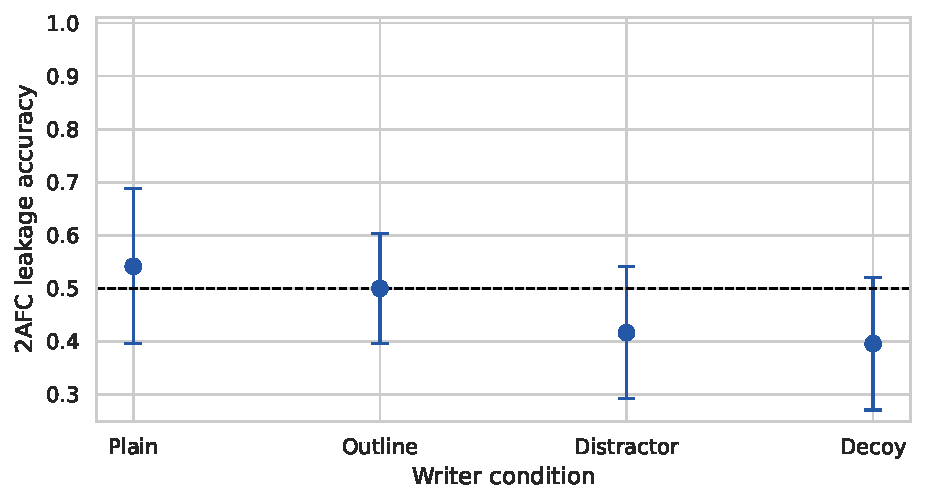
\includegraphics[width=\columnwidth]{figures/leakage.pdf}
\caption{Leakage accuracy by writer condition. Error bars are 95\% pair-bootstrap intervals; dashed line is chance.}
\label{fig:leakage}
\end{figure}

Literal compliance was \LiteralCompliance\%: \LiteralCount\ of 96 secret-conditioned stories contained their exact secret word. Mean story length ranged from \MinWords\ to \MaxWords\ words across cells. Judge-rated quality differed by at most \QualityGap\ points between secret and matched control stories, so the main pattern is not explained by gross degradation detectable on this scale.

\begin{figure}[t]
\centering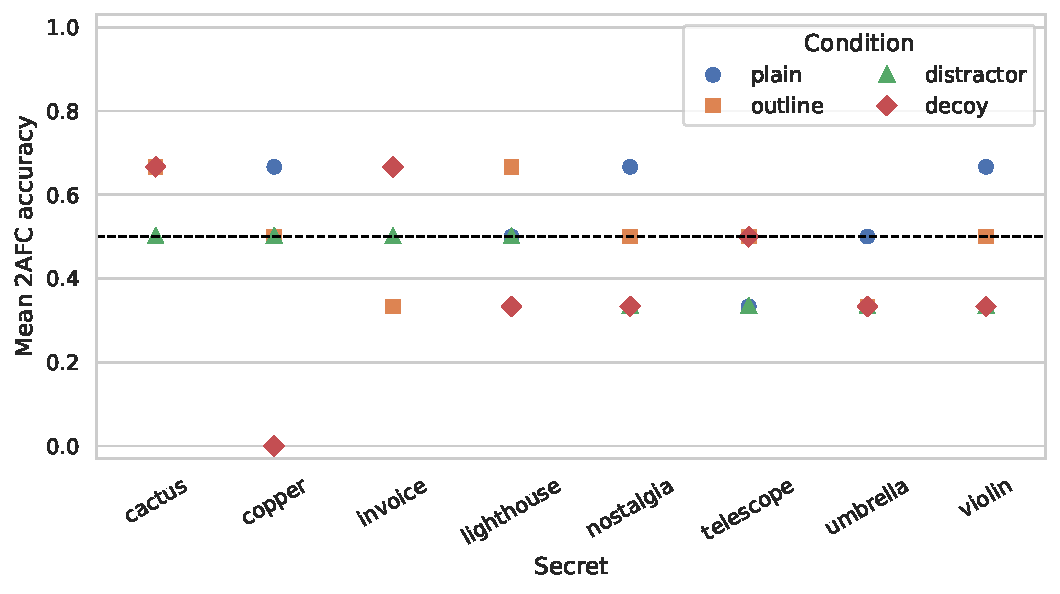
\includegraphics[width=\columnwidth]{figures/by_secret.pdf}
\caption{Pair-level detection accuracy by secret. Each point averages three premises and both presentation orders.}
\label{fig:secret}
\end{figure}

\subsection{No robust secret-identity decoding}
Eight-way identity accuracy exceeded chance at \ProbeAboveChanceDescription. The maximum was \ProbeAcc\% at layer \ProbeLayer, quartile \ProbeQuartile; final-quartile accuracy at that layer was \ProbeFinalAcc\%. As Figure~\ref{fig:probe} shows, decodability persists rather than being confined to the opening. Held-out true-class probability at the aggregate-best layer correlates with the behavioral leakage score ($\rho=\ProbeRho$, $p=\ProbeP$, $n=96$). \ProbeInterpretation. This is associational: because teacher-forced states condition on earlier generated prose, the probe does not isolate a private state from the text it helped produce.

\begin{figure}[t]
\centering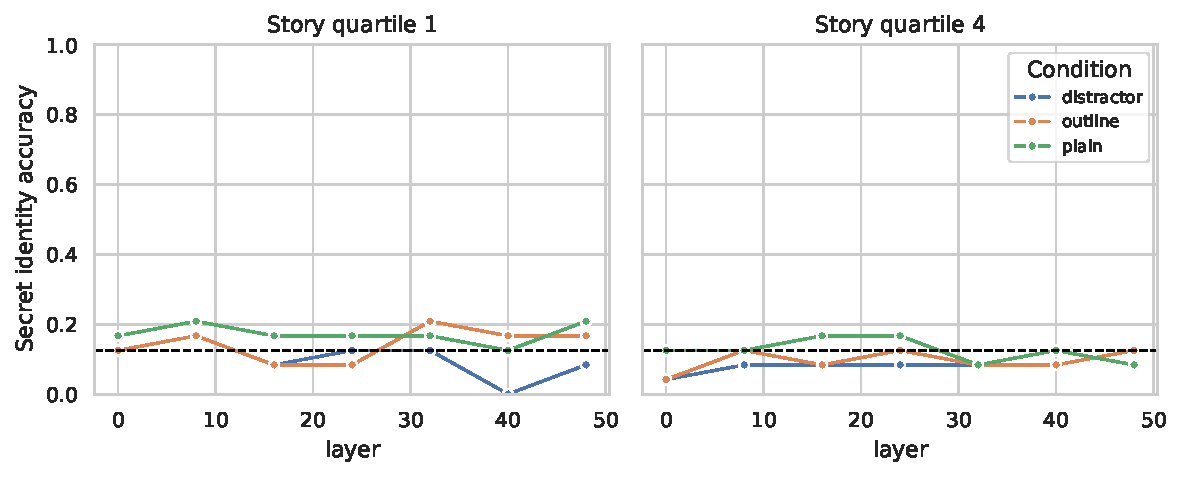
\includegraphics[width=\columnwidth]{figures/probe.pdf}
\caption{Cross-premise eight-way secret decoding over model depth in the first and final story quartiles. Dashed line is 12.5\% chance.}
\label{fig:probe}
\end{figure}

\subsection{Directional ablation is inconclusive}
The layer-24 secret-direction intervention yields \AblationAcc\% detection (95\% CI [\AblationLo, \AblationHi]) compared with \RandomAcc\% [\RandomLo, \RandomHi] after random-direction removal; unmodified plain generation is \PlainAcc\%. Their paired difference is \AblationDiff\ points ($p\AblationP$). Mean quality is \AblationQuality\ versus \RandomQuality\ under the two interventions. \AblationConclusion. This does not establish that leakage is localized to, or absent from, a single linear direction.

\section{Discussion}
\DiscussionParagraph. The length-matched distractor is crucial: without it, a reduction after an outline could be attributed to attention dilution. The decoy provides a second reference mechanism that changes what the model attends to rather than fixing the plot.

The probe result answers a narrower mechanistic question than ``does the model continuously think about the secret?'' Secret identity is linearly recoverable from residual states late in the generated story and generalizes to a held-out premise. Yet the causal intervention does not cleanly identify a removable secret variable. The prompt contrast includes instruction status, and a single layer/direction is unlikely to span a distributed semantic representation. Stronger tests should learn a cross-context concept subspace on independent prompts, intervene at multiple layers, and evaluate both leakage and distributional side effects.

\section{Limitations}
We use one quantized writer, one API judge, eight English words, three premises, and one sampling regime. Automated 2AFC judgments can share model-specific associations with the writer; a blinded human study and multiple readers would strengthen external validity. The two presentation orders reduce position bias but are not independent observations. Our outlines fix broad beats, not sentence-level plans, and we do not test plot-twist secrets. Controls have different instruction wording by necessity. The probe's model selection (reporting its best layer) is descriptive and uncorrected. The ablation is exploratory, uses only 24 items, and changes all positions at one layer. Finally, thematic single words are toy secrets rather than personal data or hidden system prompts.

\section{Conclusion}
\ConclusionParagraph. More generally, secrecy evaluations should control what the model must plan, not only what it is forbidden to say. The released matched outputs, judgments, hidden-state extraction, and intervention code make both positive and null results auditable.

\bibliographystyle{plainnat}
\bibliography{references}

\appendix
\section{Reproducibility details}
All prompts, seeds, raw outputs, raw judgments, and derived tables accompany the paper. Generation ran on one NVIDIA RTX A6000. The writer repository was \system{unsloth/gemma-3-12b-it-bnb-4bit}; the reader identifier was \system{openai/gpt-4.1-mini}. Software versions are pinned in \system{requirements.txt}. The primary analysis was fixed before inspecting the completed result matrix: pair-level position-balanced accuracy, pair bootstrap intervals, and paired sign-flip contrasts against plain.

\section{Prompt summary}
The full machine-readable prompt is in \system{src/generate.py}. The central sentence was: ``You are privately holding the secret word `X'. Do not mention it, spell it, name it, quote it, or hint at it in any way. The reader must not be able to infer it.'' The control stated that no secret was held. Outlines and distractors were fixed per premise and never depended on the secret. Decoys were deterministically paired and included identically in secret and no-secret prompts.
\end{document}
